\documentclass[sigconf]{acmart}

\usepackage{mathtools}
\usepackage{booktabs}

\setcopyright{none}
\settopmatter{printacmref=true}
\renewcommand\footnotetextcopyrightpermission[1]{}

\newtheorem{theorem}{Theorem}
\newtheorem{proposition}{Proposition}
\theoremstyle{remark}
\newtheorem{remark}{Remark}

\newcommand{\Matern}{\mathcal M}
\newcommand{\E}{\mathbb E}
\newcommand{\R}{\mathbb R}
\newcommand{\tr}{\operatorname{tr}}

\title{SupportShift: A Theory-Linked Spatial Simulation Benchmark
for Ignored Matérn Observation Support}

\author{Sasha Cui}
\affiliation{%
  \institution{Independent researcher}
  \city{New Haven}
  \state{Connecticut}
  \country{United States}}

\acmConference[GeoSim '26]{9th ACM SIGSPATIAL International Workshop on
Geospatial Simulation}{November 3, 2026}{Riverside, California, USA}
\acmYear{2026}
\copyrightyear{2026}
\acmDOI{}
\acmISBN{}

\begin{abstract}
Spatial measurements often represent pixels, footprints, or local averages but
are fitted as point observations. We introduce \emph{SupportShift}, a
parameterized synthetic benchmark that separates the physical covariance
parameter, the population Kullback--Leibler (KL) target, and finite-sample
estimation error under this support misspecification. Its analytic anchor is a
stationary Matérn Gaussian field in \(\R^d\) observed through a compact
symmetric averaging kernel of bandwidth \(h\). For a fixed nonzero-lag
two-point likelihood with known smoothness \(\nu\), the naive inverse-range
shift has order \(h^{2\nu}\) for \(0<\nu<1\),
\(h^2\log(1/h)\) at \(\nu=1\), and \(h^2\) for \(\nu>1\). Explicit
coefficients prove range inflation for every fixed \(\nu>0\) at sufficiently
small support and yield a directional \(h^2\) contrast for elongated support.
For \(N\) independent \(p\)-dimensional Gaussian fields and a deterministic
finite covariance library, a simultaneous likelihood certificate scales as
\(\sqrt{\log(M)/(Np)}+\log(M)/(Np)\) under relative spectral control; spatial
dependence within each field is unrestricted. Four reproducible tracks pair
these statements with deterministic quadrature, finite-grid likelihoods,
directional support, and growing-\(p\) replicated fields. The benchmark exposes
a sharp failure mode: likelihood noise can vanish while a point-support fit
concentrates around the wrong range target.
\end{abstract}

\begin{CCSXML}
<ccs2012>
 <concept>
  <concept_id>10002950.10003714.10003715</concept_id>
  <concept_desc>Mathematics of computing~Probabilistic representations</concept_desc>
  <concept_significance>500</concept_significance>
 </concept>
 <concept>
  <concept_id>10002950.10003648.10003649</concept_id>
  <concept_desc>Mathematics of computing~Probability and statistics</concept_desc>
  <concept_significance>500</concept_significance>
 </concept>
</ccs2012>
\end{CCSXML}

\ccsdesc[500]{Mathematics of computing~Probability and statistics}
\ccsdesc[300]{Mathematics of computing~Probabilistic representations}

\keywords{Matérn covariance, change of support, Gaussian random field,
high-dimensional probability, spatial simulation benchmark, misspecified likelihood}

\begin{document}
\maketitle

\section{Introduction}

Values recorded on pixels, grid cells, or after kernel preprocessing are local
aggregates of an underlying spatial field. Change-of-support models account for
this by integrating the latent process over the measurement support
\cite{gelfand2001support,chacon2024change,tanaka2019aggregated,zheng2026fusion}.
A common shortcut instead assigns each aggregate to a declared center and fits a
point-support covariance. Relative to the latent parameters, the support is then
misinterpreted. A single two-point covariance can still be matched exactly by
different variance and decay parameters; a multi-lag likelihood is genuinely
misspecified and selects a Kullback--Leibler (KL) projection
\cite{bachoc2018misspecified}.

This qualitative fact leaves quantitative and experimental questions. How
quickly does the pseudo-parameter move as support shrinks? Does the rate depend
on Matérn smoothness? Can directional support masquerade as directional range?
Finally, does increasing dimension or replication remove the error, or merely
make a wrong population target more precise? The first answer is not an ordinary
second-order Taylor expansion: the Matérn covariance changes regularity at the
origin as smoothness crosses one.

Block covariance and regularized variograms are classical
\cite{chiles2012geostatistics,gelfand2001support,gotway2002incompatible}.
Modern aggregated-GP and INLA--SPDE methods likewise put the support operator
inside the observation model \cite{tanaka2019aggregated,zheng2026fusion}.
Convolution and covariance anisotropy can also be confounded
\cite{clifford2006yield,paciorek2006nonstationary}. Generic misspecified-GP
theory supplies the KL framework \cite{bachoc2018misspecified}, while Gaussian
quadratic-form concentration is standard
\cite{laurent2000quadratic,hsu2012quadratic}. Table~\ref{tab:literature}
separates these known ingredients from our claims.

We contribute a theorem-linked benchmark rather than a new generic
change-of-support method:

\begin{itemize}
  \item We derive an all-smoothness, \(d\)-dimensional fixed-lag phase law
  with explicit coefficients and a universal small-support range direction.
  \item We derive a directional \(h^2\) apparent-range contrast for linearly
  transformed support. The qualitative convolution--anisotropy link is not
  claimed as new.
  \item We certify finite-library likelihood selection for \(N\) independent
  \(p\)-dimensional Gaussian fields without assuming independent spatial
  coordinates.
  \item SupportShift turns the theorem into four reusable synthetic tracks:
  a continuous phase oracle, finite-grid likelihoods, directional support, and
  growing-\(p\) replicated fields, with deterministic seeds and numerical gates.
\end{itemize}

The phase theorem is pairwise; full-grid targets are computed, not asserted to
share its coefficient. The high-dimensional experiment grows domain at fixed
lattice spacing and uses independent replicated fields. We do not claim
separate fixed-domain consistency of Matérn variance and range, which would
conflict with microergodicity results
\cite{zhang2004inconsistent,kaufman2013range}.

\begin{table*}[t]
\centering
\caption{Nearest known ingredients and the narrower SupportShift addition.}
\label{tab:literature}
\begin{tabular}{p{0.28\textwidth}p{0.29\textwidth}p{0.35\textwidth}}
\toprule
Literature & Established result & Addition studied here \\
\midrule
Change of support and block covariance
\cite{chiles2012geostatistics,gelfand2001support,tanaka2019aggregated}
& Integrate the latent covariance over known observation supports
& Explicit small-support Matérn \emph{point-fit pseudo-range} phase law \\
Misspecified GP likelihood \cite{bachoc2018misspecified}
& Population KL pseudo-target under covariance misspecification
& Closed direction, rate, and coefficient for ignored support \\
Convolution and anisotropy \cite{clifford2006yield,paciorek2006nonstationary}
& Support/convolution can create anisotropic covariance
& Leading directional apparent-range contrast \\
Gaussian quadratic forms \cite{laurent2000quadratic,hsu2012quadratic}
& Nonasymptotic concentration of Gaussian quadratic forms
& Direct certificate for the benchmark's structured covariance library \\
Spatial benchmarks \cite{heaton2019competition}
& Shared synthetic data and auditable method comparisons
& Support-specific generator with analytic targets and pass/fail gates \\
\bottomrule
\end{tabular}
\end{table*}

\section{Model and exact pair target}

Let \(Y=\{Y(t):t\in\R^d\}\) be a mean-zero stationary Gaussian field with
\begin{equation}
  C(r)=v\Matern_\nu(\alpha\lVert r\rVert),\qquad
  \Matern_\nu(x)=\frac{2^{1-\nu}}{\Gamma(\nu)}x^\nu K_\nu(x),
  \label{eq:cov}
\end{equation}
where \(v,\alpha,\nu>0\) and \(\Matern_\nu(0)=1\). Thus \(\alpha\) is inverse
range. Let \(k\) be a symmetric probability density supported on
\(B(0,L)\), set \(k_h(u)=h^{-d}k(u/h)\), and observe
\begin{equation}
  Z_h(t)=\int k_h(u)Y(t-u)\,du.
\end{equation}
For independent \(U,V\sim k\), write \(D=U-V\),
\(\Sigma_k=\E(UU^\top)\), \(T_k=\tr(\Sigma_k)\), and
\(m_q=\E\lVert D\rVert^q\). Then \(m_2=2T_k\), and stationarity gives
\begin{equation}
  C_h(r)=v\E\!\left[\Matern_\nu\{\alpha\lVert r+hD\rVert\}\right].
  \label{eq:smoothcov}
\end{equation}
Assume \(T_k>0\).

Fix \(r=Re\), \(R>0\), and \(\lVert e\rVert=1\). A naive point-support pair
model with known \(\nu\) and unknown variance and inverse range uses
\begin{equation}
  v^\dagger
  \begin{pmatrix}
  1 & \Matern_\nu(\alpha^\dagger R)\\
  \Matern_\nu(\alpha^\dagger R)&1
  \end{pmatrix}.
\end{equation}
The smoothed two-by-two covariance lies in this family. Moreover,
\(0<\rho_h(r)<1\): positivity follows from \(k\geq0\) and
\(\Matern_\nu>0\), while strict inequality follows from the positive smoothed
spectral density near the origin. Hence the exact Gaussian KL target is
\begin{equation}
  v_h^\dagger=C_h(0),\qquad
  \Matern_\nu(\alpha_h^\dagger R)=\rho_h(r)
  :=\frac{C_h(r)}{C_h(0)}.
  \label{eq:target}
\end{equation}
It is unique because
\begin{equation}
  \Matern_\nu'(x)
  =-\frac{2^{1-\nu}}{\Gamma(\nu)}x^\nu K_{\nu-1}(x)<0.
  \label{eq:deriv}
\end{equation}
On a fixed lattice and increasing rectangular F{\o}lner domains, a
pair-composite estimator converges to this target under a compact parameter
space, target uniqueness and interiority, correlations bounded away from one,
and the usual continuity and integrable-envelope conditions for a uniform
ergodic law. Dependence among overlapping pairs requires Godambe uncertainty;
it does not change this population target.

\section{Smoothness-dependent phase law}

Put \(z=\alpha R\), \(a_k(e)=e^\top\Sigma_ke\), and
\begin{equation}
 B_{\nu,k}(r)=\alpha^2\left[
 a_k(e)\Matern_\nu''(z)
 +\{T_k-a_k(e)\}\frac{\Matern_\nu'(z)}{z}\right].
\end{equation}

\begin{proposition}[Fixed nonzero lag]
Uniformly for \(r\) in a compact annulus bounded away from zero, for
\(h\leq\lVert r\rVert/(4L)\), and for \(\alpha\) in a compact subset of
\((0,\infty)\),
\begin{equation}
  \frac{C_h(r)}{v}
  =\Matern_\nu(\alpha\lVert r\rVert)+h^2B_{\nu,k}(r)+O(h^4).
  \label{eq:lag}
\end{equation}
\end{proposition}

At zero lag, the Matérn origin expansion produces a phase transition.

\begin{theorem}[Matérn support phase law]
Fix \(\nu>0\).
Let
\[
c_\nu=\frac{\Gamma(1-\nu)}
{\nu2^{2\nu}\Gamma(\nu)}>0,\qquad 0<\nu<1.
\]
Under the preceding assumptions, as \(h\downarrow0\),
\begin{align}
\frac{C_h(0)}v
&=1-c_\nu m_{2\nu}(\alpha h)^{2\nu}+O(h^2),
&&0<\nu<1, \label{eq:vrough}\\
&=1-\frac{m_2}{2}(\alpha h)^2\log\{1/(\alpha h)\}+O(h^2),
&&\nu=1, \label{eq:vone}\\
&=1-\frac{m_2}{4(\nu-1)}(\alpha h)^2+o(h^2),
&&\nu>1. \label{eq:vsmooth}
\end{align}
The pseudo-decay in \eqref{eq:target} satisfies
\begin{align}
\alpha_h^\dagger-\alpha
&=\frac{\Matern_\nu(z)c_\nu m_{2\nu}\alpha^{2\nu}}
{R\Matern_\nu'(z)}h^{2\nu}
+O\!\left(h^{\min(4\nu,2)}\right),
&&0<\nu<1, \label{eq:arough}\\
\alpha_h^\dagger-\alpha
&\sim\frac{m_2\Matern_1(z)\alpha^2}
{2R\Matern_1'(z)}h^2\log(1/h),
&&\nu=1, \label{eq:aone}\\
\alpha_h^\dagger-\alpha
&=\frac{A_{\nu,k}(r)}{R\Matern_\nu'(z)}h^2+\mathcal R_\nu(h),
&&\nu>1, \label{eq:asmooth}
\end{align}
where
\begin{align}
A_{\nu,k}(r)
&=\alpha^2\{(2\nu-2)a_k(e)+T_k\}G_\nu(z)>0,\\
G_\nu(z)
&=\frac{\Matern_\nu(z)}{2\nu-2}+\frac{\Matern_\nu'(z)}z\\
&=\frac{2^{1-\nu}}{\Gamma(\nu)}
\frac{z^\nu K_{\nu-2}(z)}{2\nu-2}>0,
\end{align}
and \(\mathcal R_\nu(h)=O(h^{2\nu})\) for \(1<\nu<2\),
\(O\{h^4\log(1/h)\}\) for \(\nu=2\), and \(O(h^4)\) for \(\nu>2\).
For fixed \(\nu\), the remainders are uniform over compact positive decay sets
and lag annuli bounded away from zero, but not as \(\nu\) approaches one or two.
Consequently, for every \(\nu>0\) and all sufficiently small \(h>0\),
\[
v_h^\dagger<v,\qquad \rho_h(r)>\Matern_\nu(\alpha R),\qquad
\alpha_h^\dagger<\alpha.
\]
\end{theorem}

\begin{proposition}[Directional support contrast]
Let \(\Delta_e(h)=\alpha-\alpha_h^\dagger(e)\). For two unit lag
directions \(e_1,e_2\), under the theorem assumptions,
\begin{equation}
 \Delta_{e_1}(h)-\Delta_{e_2}(h)
 =\frac{\alpha^2\{a_k(e_1)-a_k(e_2)\}}R
  \frac{K_{\nu-2}(z)}{K_{\nu-1}(z)}h^2+o(h^2).
 \label{eq:direction}
\end{equation}
The formula holds for every \(\nu>0\). When \(\nu\leq1\), it is lower
order than the direction-independent leading shift in the phase theorem.
\end{proposition}

For the benchmark's transformed product Epanechnikov smoother
\(Z_{h,A}(t)=\int k(u)Y(t-hAu)\,du\),
\(\Sigma_k=AA^\top/5\). We parameterize its principal singular-value aspect
ratio \(\varrho\geq1\) while holding \(\tr(\Sigma_k)\) fixed using
\begin{equation}
 A_\varrho=\sqrt{\frac{2}{\varrho+\varrho^{-1}}}
 \operatorname{diag}(\sqrt\varrho,\varrho^{-1/2}).
 \label{eq:transform}
\end{equation}
For \(\nu>1\), the ratio of the major- to minor-axis leading shift
coefficients is
\begin{equation}
 \frac{(2\nu-1)\varrho^2+1}{\varrho^2+2\nu-1}.
 \label{eq:aspectratio}
\end{equation}
Thus elongated measurement support alone can induce directional apparent
range, even though the latent Matérn covariance is isotropic.

\begin{remark}
The fitted lag \(R\) is fixed and bounded away from zero. If \(R=ch\), the
nonzero-lag expansion is no longer uniform and the relative displacement need
not vanish.
\end{remark}

Thus ignored support inflates inferred range. The sign is not an assumption:
for \(\nu>1\), it follows from positivity of \(K_{\nu-2}\) in the displayed
identity. For an isotropic kernel,
\(A_{\nu,k}(r)=\sigma_k^2\alpha^2(2\nu+d-2)G_\nu(z)\).

\subsection{Proof sketch}

Let \(f_\alpha(x)=\Matern_\nu(\alpha\lVert x\rVert)\). At a nonzero lag,
fourth-order Taylor expansion is uniform. Symmetry and
\(\E(DD^\top)=2\Sigma_k\) cancel odd terms, including the cubic term, and yield
\eqref{eq:lag}. At zero,
the noninteger Bessel expansion is
\begin{equation}
\Matern_\nu(x)=
\sum_{j\geq0}\frac{(x^2/4)^j}{j!(1-\nu)_j}
+\frac{\Gamma(-\nu)x^{2\nu}}{2^{2\nu}\Gamma(\nu)}
\sum_{j\geq0}\frac{(x^2/4)^j}{j!(1+\nu)_j}.
\end{equation}
Taking expectations at \(x=\alpha h\lVert D\rVert\) proves
\eqref{eq:vrough} and \eqref{eq:vsmooth}. At \(\nu=1\),
\[
\Matern_1(x)=1+\frac{x^2}{2}
\{\log(x/2)+\gamma_{\rm E}-1/2\}
+O\{x^4(1+|\log x|)\},
\]
which proves \eqref{eq:vone}. Divide \eqref{eq:lag} by the relevant variance
expansion and expand the inverse of
\(\alpha\mapsto\Matern_\nu(\alpha R)\). This gives
\eqref{eq:arough}--\eqref{eq:asmooth}. For \(\nu>1\), the Matérn differential
equation and the recurrence
\[
K_\nu(z)=K_{\nu-2}(z)+2(\nu-1)K_{\nu-1}(z)/z
\]
reduce the normalized-correlation coefficient to \(A_{\nu,k}(r)\), proving its
sign. Full transition constants and an exact exponential benchmark are in the
reproducible technical manuscript.

At the remaining integer transition,
\[
\Matern_2(x)=1-\frac{x^2}{4}
+x^4\left\{\frac{3}{64}
-\frac{\log(x/2)+\gamma_{\rm E}}{16}\right\}
+O\{x^6(1+|\log x|)\}.
\]
For fixed \(\nu>2\), four-times differentiability yields
\(\Matern_\nu(x)=1-x^2/\{4(\nu-1)\}+O(x^4)\). These formulas, and the
fractional term for \(1<\nu<2\), give the three stated smooth-regime
remainders after division and inverse expansion.

\section{Finite-grid support-aware likelihood}

The theorem covers translation-invariant interior averaging. For a finite
simulation, let \(X_{\rm in}\) denote raw sites and let
\(S_h\in\R^{m\times n}\) be a rectangular row-stochastic observation operator.
With noise present before smoothing,
\begin{equation}
y=S_h\{Y(X_{\rm in})+\epsilon\},\qquad
\epsilon\sim N(0,\tau^2I_n),
\end{equation}
the support-aware covariance is
\begin{equation}
\Sigma_{\rm corr}(\alpha)
=S_h\{K_\alpha(X_{\rm in},X_{\rm in})+\tau^2I_n\}S_h^\top.
\label{eq:corr}
\end{equation}
The naive declared-center point-support covariance is instead
\begin{equation}
\Sigma_{\rm naive}(\alpha)
=K_\alpha(X_{\rm out},X_{\rm out})+\tau^2I_m.
\label{eq:naive}
\end{equation}
Besides ignoring support, \eqref{eq:naive} treats pre-smoothing noise as
independent post-smoothing noise.

With variance, smoothness, and nugget fixed, the finite-design KL target
minimizes
\begin{equation}
Q_n(\alpha)=\frac12\left[
\log\det\Sigma(\alpha)+
\tr\{\Sigma(\alpha)^{-1}\Sigma_0\}\right].
\label{eq:kl}
\end{equation}
The corrected family contains \(\Sigma_0\) when the operator and fixed nuisance
parameters are correctly specified and decay is identifiable; the naive family
generally does not. Our primary experiment sets \(\tau=0\), isolating field
support from noise-timing misspecification. A separate \(\tau^2=0.05\) run is
retained only as a combined-misspecification artifact. Rectangular \(S_h\) is
intentional: an invertible square,
parameter-independent transform may merely change coordinates, whereas
aggregation reduces raw sites to fewer supported outputs.

Boundary row normalization is outside the interior theorem. If two
location-dependent scaled kernels have means \(\mu_s\) and \(\mu_t\), then
\[
C_{h,s,t}(r)=C(r)+h\nabla C(r)^\top(\mu_s-\mu_t)+O(h^2).
\]
A truncated kernel can therefore create a first-order term and destroy
stationarity; the interior theorem gives no boundary sign guarantee. We include
one boundary and one fixed irregular design as illustrations, not as a boundary
scaling study.

\subsection{Finite-library high-dimensional certificate}

The growing-\(p\) benchmark jointly varies variance and decay on a deterministic
finite grid. The following standard quadratic-form consequence explains which
part of its error can shrink with information; it is supporting machinery, not
a new concentration inequality.

\begin{proposition}[Gaussian finite-library certificate]
Let \(X_1,\ldots,X_N\overset{\mathrm{iid}}\sim N_p(0,\Sigma_0)\), and let
\(\{\Sigma_\theta:\theta\in\mathcal G\}\) be a deterministic library of
\(M\) positive-definite covariances. Define
\begin{align}
 \widehat\Sigma_N&=N^{-1}\sum_{i=1}^NX_iX_i^\top,\\
 \widehat L_N(\theta)&=\frac1{2p}\left\{\log\det\Sigma_\theta+
 \tr(\Sigma_\theta^{-1}\widehat\Sigma_N)\right\},
 \label{eq:empiricalrisk}\\
 L(\theta)&=\E\widehat L_N(\theta),\qquad
 A_\theta=\Sigma_0^{1/2}\Sigma_\theta^{-1}\Sigma_0^{1/2}.
\end{align}
For \(t=\log(2M/\delta)\), with probability at least \(1-\delta\),
simultaneously for every \(\theta\in\mathcal G\),
\begin{equation}
 |\widehat L_N(\theta)-L(\theta)|\leq
 \frac{\lVert A_\theta\rVert_F}{p}\sqrt{\frac tN}
 +\frac{\lVert A_\theta\rVert_{\rm op}}p\frac tN
 =:u_\theta.
 \label{eq:certificate}
\end{equation}
If \(\widehat\theta\) and \(\theta^\star\) minimize the empirical and
population criteria, respectively, then
\begin{equation}
 L(\widehat\theta)-L(\theta^\star)
 \leq2\max_{\theta\in\mathcal G}u_\theta.
 \label{eq:erm}
\end{equation}
Moreover, \(L(\theta)\) differs from
\(p^{-1}D_{\rm KL}\{N(0,\Sigma_0)\Vert N(0,\Sigma_\theta)\}\) by a
candidate-independent constant.
\end{proposition}

To prove \eqref{eq:certificate}, write \(X_i=\Sigma_0^{1/2}Z_i\), stack the
standard Gaussian vectors, and apply the Gaussian quadratic-form inequality to
\(I_N\otimes A_\theta\). Its Frobenius and operator norms are
\(\sqrt N\lVert A_\theta\rVert_F\) and
\(\lVert A_\theta\rVert_{\rm op}\); division by \(2Np\) and a union bound
give the displayed constants \cite{laurent2000quadratic,hsu2012quadratic}.
The ERM result is the usual three-term comparison through
\(\widehat L_N\).

No coordinate independence is used: all within-field spatial dependence is in
\(\Sigma_0\). If
\(c\Sigma_0\preceq\Sigma_\theta\preceq C\Sigma_0\) uniformly, then
\begin{equation}
 \max_\theta u_\theta\leq c^{-1}\left\{
 \sqrt{\frac{\log(2M/\delta)}{Np}}
 +\frac{\log(2M/\delta)}{Np}\right\}.
 \label{eq:np-rate}
\end{equation}
This conditional rate does not imply separate fixed-domain range and variance
consistency: relative spectra or parameter curvature may deteriorate with
\(p\). The benchmark therefore reports the actual matrix norms and the exact
candidate-specific radius.

\section{Synthetic validation}

\subsection{Continuous phase oracle}

We used a two-dimensional product Epanechnikov density, \(\alpha=R=1\),
tensor Gauss--Legendre order 96, 18 bandwidths from 0.003 to 0.3, and
\(\nu\in\{0.25,0.5,0.75,1,1.5,2.5\}\). The density of each coordinate of
\(D\) is available in closed form, so \eqref{eq:smoothcov} is evaluated by
deterministic quadrature. We solved \eqref{eq:target} by monotone root finding.
Repeating at orders 64 and 128 changed pseudo-decay by at most
\(4.4\times10^{-8}\) and \(5.2\times10^{-9}\), respectively, relative to
order 96.

All 108 shifts \(\alpha-\alpha_h^\dagger\) were positive. For smoothness 0.25,
0.5, and 0.75, log--log slopes over the six smallest bandwidths were 0.515,
0.999, and 1.468, versus theoretical powers 0.5, 1, and 1.5. The raw
slope at \(\nu=1\) was 1.817, reflecting the logarithmic modifier. Slopes for
\(\nu=1.5\) and 2.5 were 1.994 and 2.000. At the smallest bandwidth, ratios of
the exact shift to the full theorem leading term were 1.021, 1.000, 0.958,
1.059, 0.997, and 1.000 in increasing order of \(\nu\).

\begin{figure*}[t]
\centering
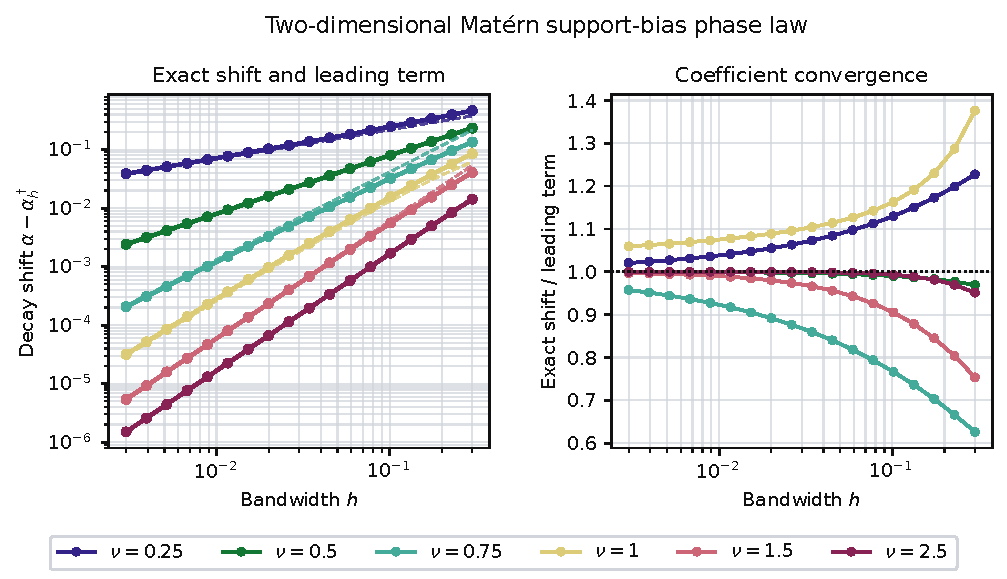
\includegraphics[width=0.86\textwidth]{figures/phase_law.pdf}
\Description{Two panels compare exact Matérn inverse-range shifts with their
leading asymptotic terms over smoothing bandwidth on logarithmic axes.}
\caption{Continuous two-dimensional pseudo-decay shift. Left: exact shifts
(solid) and theorem leading terms with explicit coefficients (dashed). Right:
their ratio, which approaches one as \(h\downarrow0\).}
\label{fig:phase}
\end{figure*}

\subsection{Finite-grid full likelihood}

The core design uses a \(19\times19\) input lattice with spacing 0.25 and every
second site as a candidate output center, trimmed by 0.75 in each coordinate.
We set \(v=\alpha=1\), \(\tau^2=0\),
\(\nu\in\{0.5,1,1.5,2.5\}\), and \(h\in\{0,0.3,0.5,0.7\}\).
Radial Epanechnikov rows are normalized exactly. Stress designs retain boundary
centers, perturb each coordinate uniformly in \([-0.04,0.04]\) before clipping,
and grow one-dimensional domains from 100 to 400 raw sites. The irregular
panel is one fixed realization.

For each configuration, \eqref{eq:kl} was minimized by bounded scalar
optimization over \(\log\alpha\in[\log(0.02),\log(5)]\). Two hundred replicate
likelihoods were evaluated on a 161-point log-decay profile; interior minima
were refined by three-point quadratic interpolation and endpoint minima were
retained as boundary fits. Gaussian raw-observation vectors were transformed by
\(S_h\). Common random numbers were reused across bandwidths. No adaptive
diagonal jitter was added; a Cholesky or population-optimization failure would
abort the configuration and make the reducer mark the run incomplete.

The immutable run contained 21 configurations and 8,400 fits. The reducer
verified configuration hashes, row counts, and unique model--replicate keys;
independent checks covered finiteness, model labels, replicate indices, and
metadata. Across the core designs, corrected population targets
were within \(1.3\times10^{-7}\) of one. At \(h=0.7\), naive targets were
0.152, 0.414, 0.573, and 0.740 as \(\nu\) increased; Monte Carlo means were
0.151, 0.407, 0.570, and 0.738. Corrected means were 1.090, 0.990, 0.990,
and 0.994. The first was within two Monte Carlo standard errors of its target.
All six core boundary-hitting fits were retained.

\begin{figure*}[t]
\centering
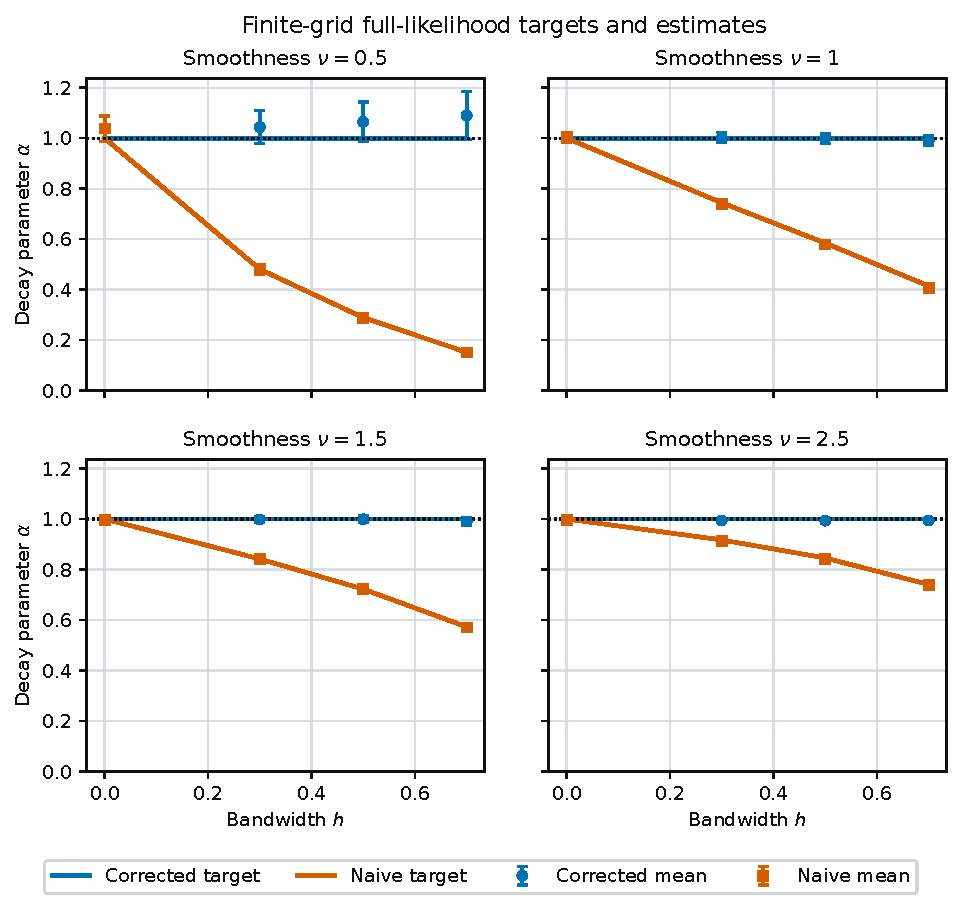
\includegraphics[width=0.84\textwidth]{figures/finite_targets.pdf}
\Description{Four panels show support-aware and naive population inverse-range
targets and Monte Carlo means over bandwidth for four Matérn smoothness values.}
\caption{Finite-design full-likelihood targets and Monte Carlo mean estimates.
Error bars show two Monte Carlo standard errors of the mean.}
\label{fig:finite}
\end{figure*}

Including boundary outputs changed both output dimension and the rough-field
naive target, from 0.152 to 0.135 at \(h=0.7\); for the fixed jittered design
the target moved from 0.289 to 0.284 at \(h=0.5\). Corrected targets remained
one. In the domain-growth check, increasing raw sites from
100 to 400 reduced corrected-estimator standard deviation from 0.529 to 0.177
and naive-estimator standard deviation from 0.151 to 0.068, while at
\(n=400\) their means were within 0.026 and 0.009 of their respective targets.

\begin{table}[t]
\centering
\caption{Finite-design results at \(h=0.7\). MCSE is for the reported mean.}
\label{tab:finite}
\begin{tabular}{llrrrr}
\toprule
$\nu$ & Model & Target & Mean & MCSE & Bound hits\\
\midrule
0.5 & Corrected & 1.000 & 1.090 & 0.047 & 3\\
0.5 & Naive & 0.152 & 0.151 & 0.004 & 0\\
1 & Corrected & 1.000 & 0.990 & 0.010 & 0\\
1 & Naive & 0.414 & 0.407 & 0.005 & 0\\
1.5 & Corrected & 1.000 & 0.990 & 0.007 & 0\\
1.5 & Naive & 0.573 & 0.570 & 0.005 & 0\\
2.5 & Corrected & 1.000 & 0.994 & 0.004 & 0\\
2.5 & Naive & 0.740 & 0.738 & 0.003 & 0\\
\bottomrule
\end{tabular}

\end{table}

\section{Discussion}

The theorem separates a standard operation from a less-studied inferential
consequence. Propagating a covariance through a known support is classical; the
new object is the parameter selected when that propagation is ignored. Rough
Matérn fields move at a fractional bandwidth power because the origin cusp
changes the variance more rapidly than fixed-lag covariance. Smooth fields move
quadratically, but a Bessel identity still fixes the sign.

The simulation has a deliberate role: it validates a theorem-linked generator,
computes nonrandom finite-design KL targets, and distinguishes misspecification
from finite-sample error. It is not a substitute for the proof. The zero-support
case verifies exact agreement, the corrected target verifies model containment,
and the boundary and irregular panels expose where the interior theorem stops.

The scope is narrow. Smoothness and support are known; nuisance parameters are
fixed in the finite study. The closed target is for a two-point criterion, while
full-grid targets are numerical. Fixed-resolution discrete smoothing does not
converge to continuous convolution merely because the domain grows. Boundary
normalization can introduce first-order terms. Joint support, smoothness,
variance, and range estimation may be weakly identified. These are future
problems, not implicit claims.

Recent finite-grid Matérn work studies discretization and edge effects without
deriving this preprocessing-support pseudo-target phase law
\cite{simons2026finite}. The defensible novelty claim is therefore limited to
the explicit all-\(\nu\) expansion and universal small-support range direction.

\section{Conclusion}

For a fixed nonzero-lag pair fit under translation-invariant interior
averaging, ignored support makes a Matérn field look more persistent than it is.
The inverse-range displacement is \(h^{2\nu}\), \(h^2\log(1/h)\), or \(h^2\),
and its leading sign is negative across fixed smoothness values, dimensions,
and compact symmetric kernels. A support-aware covariance removes the
finite-design population shift when the known operator and fixed nuisance
parameters are correctly specified and decay is identifiable. The result
supplies a theorem-level diagnostic and a reproducible simulation protocol; it
does not assert a universal sign for boundary supports or arbitrary
full-likelihood fits.

Code, manifests, and audited aggregate results are available at
\url{https://github.com/Sasha-Cui/HighDimSpatialStatistics} under the immutable
tag \texttt{paper-draft-v0.1.0}.

\bibliographystyle{ACM-Reference-Format}
\bibliography{references}

\end{document}
